% Capítulo 4
\chapter{Projeto e implementação do \textit{Walking gait}}
\label{ch:Math}

\begin{guide}
<<<<<<< HEAD
	Detalhar implementação do walking gait
\end{guide}

\begin{guide}
	Detalhar matemática dos movimentos.
\end{guide}

\section{\textit{Walking gait}}

Nesta seção detalhes arquiteturais da implementação do \textit{walking gait} serão descritos.

O \textit{walking gait} é o componente que coordena a caminhada mantendo o estado drobô, sabendo onde cada perna encontra-se e o seu estágio durante a caminhada. Desta forma, quando algum evento de perturbação, ou de ajuste, é disparado o \textit{walking gait} inicia a atualização das juntas a partir do estado atual. Assim, podemos descrever a caminhada como um evento contínuo no tempo.

Para realizar a tarefa de forma adequada, o componente faz uso de multi-processamento. Três \textit{threads} dentro do componente são responsáveis por tarefas específicas essenciais ao complemento do comportamento geral da caminhada: A \textit{thread} de rede, a \textit{thread} atualização dos motores e a \textit{thread} principal.

\subsection{\textit{Thread} principal: Da geração da trajetória até a aplicação às juntas}

\begin{figure}[h!]
	\centering
	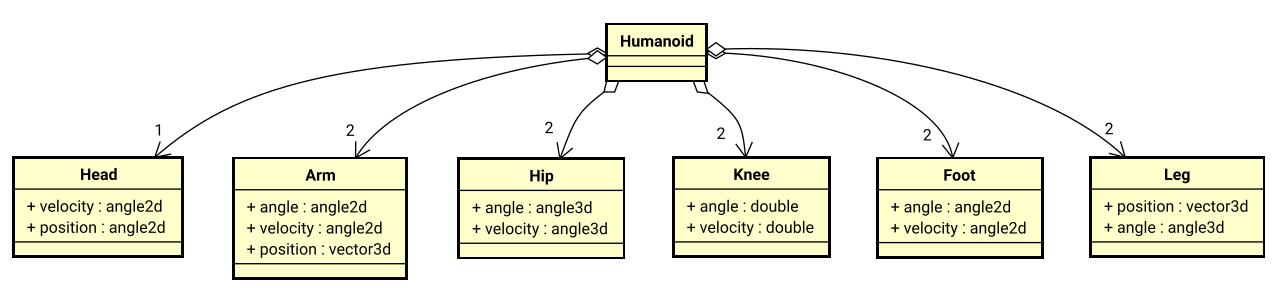
\includegraphics[scale=0.4]{imagens/svg/walkinggait-domain}
	\caption{Diagrama de domínio do \textit{walking gait}.}
	\label{fig:walkinggait:domain}
\end{figure}

A figura~\ref{fig:walkinggait:domain} mostra o diagrama de domínio das classes relevantes aos dados que o componente manipula. Nela podemos ver a classe $Humanoid$ é uma agregação de diversas outras classes que representam cada parte de Arash. É possível também observar que nas classes $Head$, $Arm$, $Hip$, $Knee$, $Foot$ existem dados ângulo e velocidade. Isso se dá por causa que componente utiliza essas informações para calcular o próximo estado do sistema em caso de algum distúrbio. Nota-se também, que a classe $Leg$ aparece de forma ambígua, já que existem as definições de $Hip$, $Knee$ e $Foot$. Porém, a classe $Leg$, representa os dados da cinemática inversa de uma perna, enquanto as demais classes guardam o estado atual das partes que representam.

Nota-se, também, a notação dos dados utilizados: $angle2d$, $angle3d$ e $vector3d$. Note que todos os tipos possuem o sufixo numérico, que indica a quantidade de dimensões aquela classe guarda, e a letra, que indica o tipo de seus dados, no caso $d$ que significa $double$. Para ângulos, $2$ dimensões significa que as dimensões $pitch$ e $roll$ são guardadas; já para $3$ dimensões as orientações $roll$, $pitch$ e $yaw$ são guardadas. Para vetores, os valores $x$, $y$ e $z$ são guardados.



\subsection{Servidor de controle}

A \textit{thread} de rede roda um servidor \textit{UDP} que aceita objetos serializandos em \textit{JSON} contendo informações de controle.



=======
	Detalhar matemática dos movimentos.
\end{guide}

\begin{draft}
	Este capítulo descreve todo o processo do cálculo das juntas.
\end{draft}

\section{Cálculo da orientação}

\begin{guide}
	Explicar os métodos utilizados para calcular a orientação.
\end{guide}

\section{Geração das trajetórias}

Para caminhar, Arash move suas juntas de uma forma sincronizada mantendo o equilíbrio. Cada passo é planejado e possíveis perturbações são compensadas o mais breve possível afim de manter a trajetória e evitar quedas. O processo de caminhada é dividido em ciclos. Cada ciclo é dado pelo movimentos de passo da perna esquerda seguido pelo movimento da perna direita. A cada momento no tempo do ciclo, as juntas do quadril, joelhos e pés tem o seu estado definido.

O método para geração da caminhada adotado possui trajetórias pré-definidas dos pés de acordo com o ciclo da caminhada. Assim, no início do processo calcula-se a posição, e orientação, do pé para cada tempo $t$.

A equação~\ref{eq:normalized_time} mostra a definição de $t$ como o tempo normalizado decorrido desde o início do ciclo. $tempo{decorrido}$ é o tempo decorrido, em milissegundos, desde o início do ciclo corrente e $tempo{total}$ é o tempo total, em milissegundos, de cada ciclo. 

\begin{equation}
t = tempo_{decorrido} / tempo_{total}
\label{eq:normalized_time}
\end{equation}

As informações geradas pela trajetória que os pés devem percorrer em cada ciclo. Essa trajetória, bem como o ciclo, são definidas no tempo gerando 4 dimensões: As 3 dimensões de posição $T_x$, $T_y$ e $T_z$; com mais um componente de rotação \textit{yaw} do pé $T_{yaw}$.

Com as informações geradas pela trajetória

Para o controlar a direção da caminhada, 3 parâmetros no controle são necessários: $V_x$, $V_y$, $V_\omega$. Onde $V_x$ é a velocidade para frente ou para trás com valores positivos para a frente; $V_y$ é a velocidade lateral com onde passos para o lado são definidos com valores positivos implicando em movimentos laterais à direita; e, finalmente, $V_\omega$ é a velocidade de rotação por passo com valores positivos indicando rotação à direita.

\begin{equation}
	-1.0 <= V_x <= 1.0
	\hspace{5mm},\hspace{5mm}
	-1.0 <= V_y <= 1.0
	\hspace{5mm},\hspace{5mm}
	-1.0 <= V_\omega <= 1.0
	\label{eq:velocities_range}
\end{equation}

Valores normalizados entre $-1.0$ e $1.0$ são utilizados para indicar as velocidades. Significando $0.0$ como o valor de velocidade nula, ou sem movimento, $1.0$ o valor de velocidade máxima para sentido ``A'' e $-1.0$ o valor de velocidade máxima porém no sentido oposto ao ``A''. Valores normalizados foram adotados para abstrair valores de velocidades absolutos já que futuras aplicações deste trabalho podem utilizar diferentes configurações de robôs. Desta forma, o controlador de comportamento pode abstrair a configuração do robô que está rodando-o e enviar velocidades relativas.

\begin{equation}
	T_{leg}(t) = 
	\begin{cases}
		
	\end{cases}
\end{equation}

\begin{guide}
	Falar sobre o processo do cálculo de forma geral.
\end{guide}

\begin{guide}
	Detalhar geração das trajetórias.
\end{guide}

\begin{guide}
	Detalhar a inverse kinematics.
\end{guide}

\begin{guide}
	Detalhar a inverse kinematics.
\end{guide}
>>>>>>> 3617d622a0e3a1343b300e7485d0c85e05d2002e

\section{Seção 1}
\label{sec:Orientacao}

Teste para símbolo

\simb[$\lambda$ (algum símbolo)]{$\lambda$}


\section{Seção 2}

Teste para abreviatura 

\abrv[IFRN -- Instituto Federal do Rio Grande do Norte]{IFRN}

\abrv[DIATINF -- Diretoria Acadêmica de Gestão e Tecnologia da
Informação]{DIATINF}
